%!TEX root = umthsmpl.tex
\chapter{Location privacy threats from advertising services}

In this chapter, I propose to study the possibility of an advertising service to be used for stalking users. I look particularly at stalking entourages and co-travelers.\footnote{We have received IRB approval for this project.}
% This chapter contains mostly proposed work, though it does contain some preliminary evaluations.

Location based services that contain mobile advertisements forward this information on to ad vendors and their clients. These include popular mobile apps such as Grindr and The Weather Channel. An advertiser can purchase advertising through an affiliate, and some affiliates allow for the client to run JavaScript in the ad. As soon as the ad is displayed on one of these apps, the script runs and in some cases sends data to the ad client along with a randomly chosen advertising ID that is unique to the device.

These mechanisms are designed to allow advertisers to target users depending on information such as location. Location information alone can allow advertisers to see where an app is used the most, and target future advertising to those locations. However, simply anonymizing location data does not protect a user from location profiling. De-anonymizing some of these users may be easy, if, for example, the user uses the app at work or at home the majority of the time. While users may trust the application they are using with location information, they likely do not trust advertising clients. As well, this information is rarely restricted by a privacy policy. Most alarmingly, anybody can be an advertiser and target any geographic location for a very low cost.

\paragraph*{Malicious intent}
There are several ways location data obtained from advertising can be used maliciously. It would be very cost effective for an attacker to determine where, for example, gay users are located, by targeting advertising in a certain city and looking at the coordinates located in residential areas of users who used gay-dating app Grindr. As well, attackers could de-anonymize a particular user and target that user to see in realtime their location or predict their location based on history; this would allow them to stalk the user or determine if the user is home. While Grindr has made the sharing of proximity optional to a user, particularly because of privacy concerns\footnote{http://www.grindr.com/blog/grindr-security/}, their location can still be found out by advertisers.

Stalking is a particularly real danger posed by advertising. If a stalker knows where a victim spends a lot of their time, and the victim happens to be using one of the popular apps that are part of the advertising network that the stalker is on, they can be followed. We explore this danger further by quantifying how many users are trackable this easily. We postulate that there are broadly three kinds of users: those who use apps at home for the most part, those who use them in a handful of places, and those who use them in many places. We principally use the advertising identifier (ad-ID) --- a randomly generated pseudonym associated with each user to build an advertising profile --- as ground truth in our experiments.
We specifically look at mobile app advertisements, which are difficult for regular users to block.

We explore also the concept of mix zones~\cite{Beresford:2004}, and how they may both be beneficial and harmful to a person's privacy. On the one hand, a user may want to choose a more populated area to use an app without being de-anonymized. On the other hand, if a person is part of an entourage that does not wish to be stalked, a single person in that entourage could compromise the entire group's privacy by using a privacy-leaking app.

\paragraph*{Experimental design}
To quantify the threat of stalking using an ad service, I plan to verify the following hypotheses.

\begin{enumerate}
\item Users can be seen multiple times, at low cost. We can manipulate how many times each user sees an ad through the bidding settings.

\item There are significant numbers of users who have 0, 1, or 2 \emph{significant stays}. Users with 0 significant stays are nomadic, users with 1 may primarily use their phones at home, users with 2 may be using them at home and work.
% \item There are significant amounts of users in each category of: homebodies, schleps, nomads. Homebodies and schleps are defined as users with 1 or 2 significant stay locations. Nomads have no geographic signature. 

\item It should be fairly easy to identify a user if she has any significant stays. There are two likely scenarios: 1. Consider a person whose details we know about (home, work), and we wish to identify. In our experiments, the identified significant stays serve as a surrogate for the outside information we'd have for the person. 2. Consider a user who has an (ad-ID) initially, and then turns off her ad-ID. Can we de-anonymize a query from that location?

\item Given a list of locations, we can identify nomads by targeting ad-IDs in certain locations. We can validate this by predicting their locations based on a public schedule using information from our advertising logs. 

\item Nomads with anonymous ids may be de-anonymized by cotravelers with de-anonymized ids. We call this the \emph{entourage attack}. This would mean that it is risky to travel in a group, if there are no strict policies on an entourage member's personal device.

\item Users can be targeted and stalked at a low financial cost to the advertiser. The cost is proportional to how easily a group can be targeted, which in turn is proportional to the population with the area of interest.
\end{enumerate}

%% TODO: how cheaply can users / protesters / targets be stalked?

%% TODO: cost?? If target an elected official, how much? How about protesters? How long, how many cities, size of entourage?

%% TODO: don't say Trump

\paragraph*{Preliminary analysis}
The existing dataset contains 350\,000 impressions from 141\,000 users. I validate the first three hypotheses using this dataset. 

% TODO: graph how many users have been subjected to x impressions and delete or change this sentence
\begin{figure}%[p]
	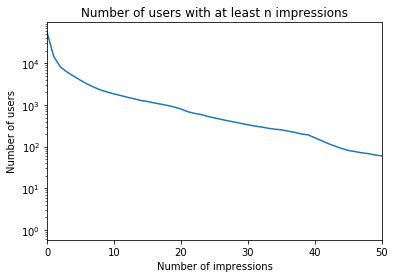
\includegraphics[width=0.5\textwidth]{graphics/numimpressions}
	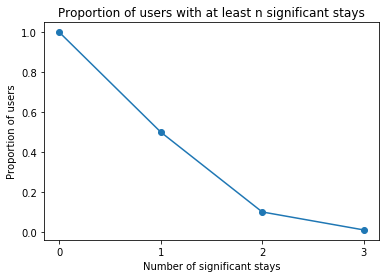
\includegraphics[width=0.5\textwidth]{graphics/sigstays}
	\caption{Left: Number of users with at least $n$ impressions. Right: Proportion of users with 10 or more impressions that have at least $n$ significant stays. }
	\label{fig:impressions}
\end{figure}

\begin{figure}%[p]
	\centering
	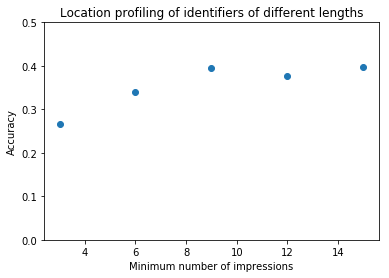
\includegraphics[width=0.7\textwidth]{graphics/impressions}
	\caption{Location profiling accuracy depending on the number of impressions}
	\label{fig:impressionprofiling}
\end{figure}

I first do a survey of types of users in our dataset. 3\% of users have 10 or more impressions (see Figure~\ref{fig:impressions} for more details). Of these users, 50\% are seen at the same one location for at least 3 times a week, 10\% at two locations, 1\% at 3 locations. There are significant amounts of users in the 1- and 2-stay categories. However, 50\% have no geographic signature.
For users with 10 or more impressions, deanonymization based on location is accurate 39\% of the time, testing and training before and after the median times of access. This means even the most naive location profiling methods are effective if we consider significant stays.

% \paragraph*{De-anonymizing identifiers}

\paragraph*{Targeting sports teams}

Despite having no geographic signature in location history, users such as elected officials, celebrities, and sports teams have public schedules. This makes them a viable target for stalking via ads. We target professional sports teams during their active season in 2017. Their travel schedule is public, and relatively unique. As well, there is a cohort of assistants and staff that may reveal the location of the team, whom may want to keep a low profile.

I plan to target NBA and NHL teams in the United States, as well as Premier League teams in the United Kingdom. I build a database of the team's true cities and times from public available information, and target those specific cities for advertising, showing each user the advertisement only once so that travelers are more likely to be reached. I then determine how well advertising identifiers correlate with known location.

There is a risk in targeting sports teams, in that they typically play in large cities, where it is more costly to target tourists or newcomers to the area. If this does not work, I will also attempt to target performers, whom have a public touring schedule and small entourage, but may travel to less populated areas.

\paragraph*{Hiding the identifier}

Users may disable advertising identifiers on their phones. However, users may still be identified by device fingerprinting, depending on the parameters of the advertising network. I plan to look at fingerprinting techniques, including location features, and how linkable they are depending on a user's location. As well, users may be deanonymized by their entourage, which may also help with linking. I also look at the feasability of location profiling co-travelers as a group.

\paragraph*{Summary of proposed work}

I will continue with this work in three directions. First, using the existing ads dataset, I will develop some methods to target users who regularly travel together or meet up. These users would be especially susceptible to the entourage attack. Second, I will collect additional data by targeting locations of sports games to de-anonymize ad-IDs of users who are part of sports teams. Finally, I will target locations of protests for ad-IDs, and follow those ad-IDs to see whether co-travelers can be identified (i.e. whether I can predict the location of someone with no advertising identifier using the location of someone previously physically close to them).

% TODO: use google ads or apple ads instead? better geotargeting?

%\begin{enumerate}
%	\item In the existing dataset, determine whether there are users who regularly travel together or meet up
%	\item In the existing dataset, determine 
%	\item Purchase ads in cities where sports games happen, and determine whether a team can be stalked using the entourage attack.
%	\item Purchase ads where protests are planned to happen.
%	\item Analyze the geolocation risk of apps and events.
%\end{enumerate}
% TODO: risk of using home wifi